\documentclass[tikz,border=7pt]{standalone}
\usepackage{iftex}
\ifPDFTeX
  \PackageError{matrix-figure}{This figure requires XeTeX or Tectonic}{Compile with xelatex or tectonic.}
\fi
\usepackage{fontspec}
\usepackage{xeCJK}
\usepackage{amsmath}
\usepackage{unicode-math}
\usepackage{xcolor}
\usepackage{tikz}
\usetikzlibrary{arrows.meta,positioning}

\providecommand{\FigureUseLocalFonts}{0}
\ifnum\FigureUseLocalFonts=1
  \setmainfont{NotoSansCJKtc-Regular.otf}[Path=\FigureSansFontPath]
  \setsansfont{NotoSansCJKtc-Regular.otf}[Path=\FigureSansFontPath,BoldFont=NotoSansCJKtc-Bold.otf]
  \setCJKmainfont{NotoSansCJKtc-Regular.otf}[Path=\FigureSansFontPath]
  \setCJKsansfont{NotoSansCJKtc-Regular.otf}[Path=\FigureSansFontPath,BoldFont=NotoSansCJKtc-Bold.otf]
  \setmathfont{STIXTwoMath.otf}[Path=\FigureMathFontPath]
\else
  \setmainfont{Noto Sans CJK TC}
  \setsansfont{Noto Sans CJK TC}
  \setCJKmainfont{Noto Sans CJK TC}
  \setCJKsansfont{Noto Sans CJK TC}
  \setmathfont{STIX Two Math}
\fi

\definecolor{FigureInk}{HTML}{253142}
\definecolor{PanelFill}{gray}{0.96}
\definecolor{RowShade}{gray}{0.86}
\definecolor{ColumnShade}{gray}{0.74}
\definecolor{ResultShade}{gray}{0.58}
\definecolor{FocusShade}{gray}{0.68}
\definecolor{GuideShade}{gray}{0.80}

\newcommand{\MatrixCell}[2]{%
  \tikz[baseline=(value.base)]{\node[fill=#1,rounded corners=0.4pt,inner sep=2.2pt,
    minimum width=1.35em,minimum height=1.35em] (value) {$#2$};}%
}
\newcommand{\RowCell}[1]{\MatrixCell{RowShade}{#1}}
\newcommand{\ColumnCell}[1]{\MatrixCell{ColumnShade}{#1}}
\newcommand{\ResultCell}[1]{\MatrixCell{ResultShade}{#1}}
\newcommand{\FocusCell}[1]{\MatrixCell{FocusShade}{#1}}

\tikzset{
  figure/.style={font=\sffamily,text=FigureInk,>={Stealth[length=3.5mm,width=2.5mm]}},
  panel/.style={draw=FigureInk,line width=0.9pt,rounded corners=1.5mm,fill=PanelFill,align=center},
  flow/.style={-{Stealth},line width=1.05pt,draw=FigureInk},
}


\begin{document}
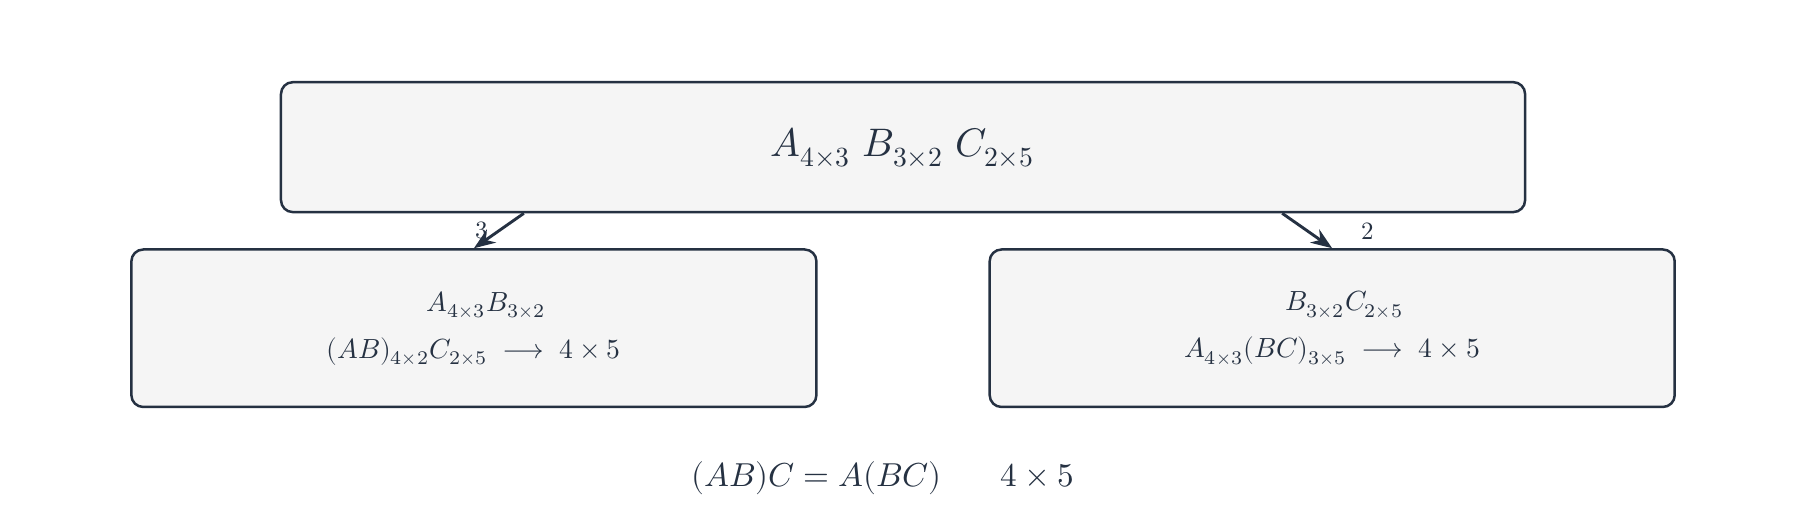
\begin{tikzpicture}[figure]
  \node[font=\bfseries\Large,align=center,text width=22cm] at (11,6.05)
    {矩陣連乘逐步核對相鄰內側階數，兩種括號位置得到同一外側階數};

  \node[panel,minimum width=15.8cm,minimum height=1.65cm,font=\Large] (start) at (11,4.65)
    {$A_{4\times3}\;B_{3\times2}\;C_{2\times5}$};

  \node[panel,minimum width=8.7cm,minimum height=2.0cm,align=center] (left) at (5.55,2.35)
    {先算 $A_{4\times3}B_{3\times2}$\\[5pt]
     $(AB)_{4\times2}C_{2\times5}\;\longrightarrow\;4\times5$};
  \node[panel,minimum width=8.7cm,minimum height=2.0cm,align=center] (right) at (16.45,2.35)
    {先算 $B_{3\times2}C_{2\times5}$\\[5pt]
     $A_{4\times3}(BC)_{3\times5}\;\longrightarrow\;4\times5$};

  \draw[flow] (start.south west) ++(3.1,0) -- (left.north)
    node[midway,left,font=\small] {先配對內側 $3$};
  \draw[flow] (start.south east) ++(-3.1,0) -- (right.north)
    node[midway,right,font=\small] {先配對內側 $2$};

  \node[font=\bfseries\large] at (11,0.45) {$(AB)C=A(BC)$，兩邊都是 $4\times5$ 階矩陣};
\end{tikzpicture}
\end{document}
